\documentclass[lettersize,journal]{IEEEtran}

% Language setting Replace `english' with e.g. `spanish' to change the document
% language
\usepackage[english]{babel}
\usepackage{caption}
\usepackage{subcaption}
\usepackage{makecell}
% \usepackage[toc,page]{appendix}
\setlength{\marginparwidth}{2cm}
\usepackage{todonotes}
\usepackage{soul}
\usepackage{pdflscape}

% Set page size and margins Replace `letterpaper' with `a4paper' for UK/EU
% standard size
\usepackage[letterpaper,top=2cm,bottom=2cm,left=3cm,right=3cm,marginparwidth=1.75cm]{geometry}

% Useful packages
\usepackage{amsmath}
\usepackage{amsfonts}
\usepackage{amssymb}
\usepackage{graphicx}
\usepackage{xspace}
\usepackage{xcolor}% http://ctan.org/pkg/xcolor
\usepackage{hyperref}
\usepackage{colortbl}
\usepackage{dsfont}

\setlength{\marginparwidth}{2cm}
\usepackage{todonotes}
\usepackage{etoolbox}
\usepackage{xargs}
\usepackage{multirow}

% Fix link colors
\hypersetup{
    colorlinks = true,
    linkcolor=red,
    citecolor=red,
    urlcolor=blue,
    linktocpage % so that page numbers are clickable in toc
}

\newcommand{\TODO}[1]{\color{red}\textsc{TODO:} #1\color{black}\xspace}
\newcommand{\TG}[1]{\color{orange}\textsc{From Tristan:} #1\color{black}\xspace}
\newcommand{\fmriprep}{fMRIPrep\xspace}
\newcommand{\fwhm}{\textsc{FWHM}}

\newcommand{\failcolor}{orange} % HEX #009E73
\newcommand{\passcolor}{green} % HEX #D55E00

\hyphenation{pre-processing}


\newcommand\Mark[2][8.4]{%
  \rlap{\tikz[baseline=(current bounding box.south)]{
        \shade[left color=\color{red}, right color=\color{green}, middle color=\color{yellow}]
               (0,0) rectangle ++(#1*#2/100,0.3);}%
  }%
}

\newtoggle{RRandRS}
\togglefalse{RRandRS} % Set it to true or false based on your requirement


\newlength{\figureWidthUM}
\newlength{\vspaceIndex}

\newcommandx{\uncertaintyMap}[5][5=false]{%
  % arguments:
  % 1: FWHM 
  % 2: subject index
  % 3: dataset
  % 4: subject
  % 5: add columns title
%   \iftoggle{RRandRS}{\setlength{\figureWidthUM}{0.2\paperheight}}{\setlength{\figureWidthUM}{0.27\paperheight}}
  \setlength{\figureWidthUM}{0.15\paperheight}
  \ifstrequal{#5}{true}{\setlength{\vspaceIndex}{-45pt}}{\setlength{\vspaceIndex}{25pt}}
  \begin{subfigure}[b]{0.01\paperwidth}
    \centering
    #2\vspace*{\vspaceIndex}
  \end{subfigure}
  \begin{subfigure}[t]{\figureWidthUM}
    \centering
    \ifstrequal{#5}{true}{IEEE (T1 intensity)}{}
    \includegraphics[width=\textwidth]{figures/sig/#1mm/ieee_#3_#4.pdf}
  \end{subfigure}
  \begin{subfigure}[t]{\figureWidthUM}
    \centering
    \ifstrequal{#5}{true}{RR (significant bits)}{}
    \includegraphics[width=\textwidth]{figures/sig/#1mm/rr_#3_#4_sig.pdf}
  \end{subfigure}
  \begin{subfigure}[t]{\figureWidthUM}
    \centering
    \ifstrequal{#5}{true}{RS (significant bits)}{}
    \includegraphics[width=\textwidth]{figures/sig/#1mm/rs_#3_#4_sig.pdf}
  \end{subfigure}
  \iftoggle{RRandRS}{%
    \begin{subfigure}[t]{\figureWidthUM}
      \centering
      \ifstrequal{#5}{true}{RR+RS (significant bits)}{}
      \includegraphics[width=\textwidth]{figures/sig/#1mm/rr.rs_#3_#4_sig.pdf}
    \end{subfigure}
  }{}
}

\newcommandx{\uncertaintyMapDiscrete}[5][5=false]{%
  % arguments:
  % 1: FWHM 
  % 2: subject index
  % 3: dataset
  % 4: subject
  % 5: add columns title
%   \iftoggle{RRandRS}{\setlength{\figureWidthUM}{0.2\paperheight}}{\setlength{\figureWidthUM}{0.27\paperheight}}
  \setlength{\figureWidthUM}{0.15\paperheight}
  \ifstrequal{#5}{true}{\setlength{\vspaceIndex}{-45pt}}{\setlength{\vspaceIndex}{25pt}}
  \begin{subfigure}[b]{0.01\paperwidth}
    \centering
    #2\vspace*{\vspaceIndex}
  \end{subfigure}
  \begin{subfigure}[t]{\figureWidthUM}
    \centering
    \ifstrequal{#5}{true}{IEEE (T1 intensity)}{}
    \includegraphics[width=\textwidth]{figures/sig/#1mm/ieee_#3_#4.pdf}
  \end{subfigure}
  \begin{subfigure}[t]{\figureWidthUM}
    \centering
    \ifstrequal{#5}{true}{RR (significant bits)}{}
    \includegraphics[width=\textwidth]{figures/sig/discrete/#1mm/rr_#3_#4_sig_discrete.pdf}
  \end{subfigure}
  \begin{subfigure}[t]{\figureWidthUM}
    \centering
    \ifstrequal{#5}{true}{RS (significant bits)}{}
    \includegraphics[width=\textwidth]{figures/sig/discrete/#1mm/rs_#3_#4_sig_discrete.pdf}
  \end{subfigure}
  \iftoggle{RRandRS}{%
    \begin{subfigure}[t]{\figureWidthUM}
      \centering
      \ifstrequal{#5}{true}{RR+RS (significant bits)}{}
      \includegraphics[width=\textwidth]{figures/sig/discrete/#1mm/rr.rs_#3_#4_sig_discrete.pdf}
    \end{subfigure}
  }{}
}


% Cluster failure: Why fMRI inferences for spatial extent lhave inflated
% false-positive https://www.pnas.org/doi/pdf/10.1073/pnas.1602413113

\title{A numerical variability approach to results stability tests and its application to neuroimaging}
\author{\IEEEauthorblockN{Yohan Chatelain\IEEEauthorrefmark{1}, Loic Tetrel\IEEEauthorrefmark{2}, Christopher J. Markiewicz\IEEEauthorrefmark{3}, Gregory Kiar\IEEEauthorrefmark{6},\\ Oscar Esteban\IEEEauthorrefmark{3}\IEEEauthorrefmark{5},  Pierre Bellec\IEEEauthorrefmark{2}\IEEEauthorrefmark{4}\IEEEauthorrefmark{7}, Tristan Glatard\IEEEauthorrefmark{1}\IEEEauthorrefmark{7}\vspace*{0.2cm}}

\IEEEauthorblockA{\IEEEauthorrefmark{1}Department of Computer Science and Software Engineering\\ Concordia University, Montreal, Quebec, Canada.}

\IEEEauthorblockA{\IEEEauthorrefmark{2} Centre de recherche de l'Institut Universitaire de Gériatrie\\ de Montréal (CRIUGM), Montréal, Québec, Canada.}

\IEEEauthorblockA{\IEEEauthorrefmark{3} Department of Psychology, Stanford University, Stanford, CA, USA.}

\IEEEauthorblockA{\IEEEauthorrefmark{4} Department of Psychology, Université de Montréal, Montréal, Québec, Canada.}

\IEEEauthorblockA{\IEEEauthorrefmark{5} Department of Radiology, Lausanne University Hospital\\ and University of Lausanne, Switzerland.}

\IEEEauthorblockA{\IEEEauthorrefmark{6} Child Mind Institute, New York City, NY, USA.}

\IEEEauthorblockA{\IEEEauthorrefmark{7} Equal contributions as last author.}

}



\begin{document}
\maketitle

\begin{abstract}
    Ensuring the long-term reproducibility of data analyses requires results stability tests to ensure that analysis results remain within acceptable variation bounds despite inevitable software updates and hardware evolutions. This paper introduces a numerical variability approach for results stability tests, which determines acceptable variation bounds using random rounding of floating-point calculations. By applying the resulting stability test to \fmriprep, a widely-used neuroimaging tool, we show that the test is sensitive enough to detect subtle updates in image processing methods while remaining specific enough to accept numerical variations within a reference version of the application. This result contributes to enhancing the reliability and reproducibility of data analyses by providing a robust and flexible method for stability testing.
\end{abstract}

\section{Introduction}

% context
The ubiquitous application of computational approaches across disciplines
  demands for the consideration of data processing as part of the measurement device
  and sets computational stability as one of the preconditions or assumptions of the data analysis.
Indeed, repeated computational processing and analyses on the same data can produce different results
  depending on the hardware and software conditions in which they are executed~\cite{gronenschild2012effects}.
Computational stability is particularly under the spotlight in neuroimaging,
  a field where software tools (e.g., \emph{FSL}~\cite{jenkinson2012fsl},
  \emph{FreeSurfer}\cite{fischl2012freesurfer}, or {\color{red} \emph{ANTs} [ref]}) % suggestion: cite also AFNI
  have built up into sophisticated instruments enabling researchers 
  to study the human brain with unprecedented detail and precision.
Unsurprisingly, the reproducibility and repeatability of neuroimaging results have been a focus of research for decades,
  yielding high-value recommendations and defining best-practices applicable across
  computational sciences {\color{red} [CITE https://doi.org/10.3389/fnins.2013.00162]}.
One thoroughly examined application is brain surface reconstruction and quantification of derived features such
  as cortical thickness, which have been shown significantly different across
  software packages ({\color{red} [CITE https://doi.org/10.1186/s12859-019-2609-8]})
  executed on the same brains.
Glatard et al. {\color{red} [Cite Tristan's paper https://doi.org/10.3389/fninf.2015.00012]}
  demonstrated operative system effects on measured cortical thickness within several software packages
  and package versions.
% neuroimaging
% We focus on the use case of neuroimaging analyses, although our method applies to data analyses more broadly. For several decades, the neuroimaging community has developed advanced software tools enabling researchers to study the human brain with unprecedented detail and precision. Neuroimaging tools now underpin scientific findings in several disciplines, and must therefore be thoroughly tested. In particular, neuroimaging studies often follow subjects over multiple years, which requires data analyses to be consistent over substantial periods.
%

Previously, computational stability has been addressed by means of random rounding (RR).
RR consists in rounding the exact result of a floating-point arithmetic operation toward the previous
  or next floating-point number~\cite{forsythe1959reprint}.
RR is equivalent to applying Monte-Carlo Arithmetic (MCA~\cite{parker1997monte}) to double-precision numbers
  with a virtual precision of 53 bits and to single-precision numbers with a virtual precision of 24 bits,
  which was shown to accurately simulate the effect of operating system updates on the structural
  MRI preprocessing pipelines of the Human Connectome Project (HCP) when applied to 
  \emph{GNU libmath}~\cite{salari2021accurate}.
The \emph{HCP pipelines} consist of tools assembled from the \emph{FSL} and \emph{Freesurfer} toolboxes.
RR is rigorously implemented in several tools including \emph{CADNA}~\cite{jezequel2008cadna},
  \emph{Verrou}~\cite{fevotte2016verrou}, and \emph{Verificarlo}~\cite{denis2016verificarlo}.
However, these tools incur substantial performance overhead that makes them hard to apply to
  compute-intensive applications.
In addition, only \emph{Verrou} supports RR instrumentation of \emph{GNU libmath}~\cite{fevotte2019debugging},
  and it does so by relying on quadruple precision, which is not scalable to entire neuroimaging pipelines.

% fmriprep
Sensitive to these computational challenges to the stability of results, 
  the developers of the \fmriprep software~\cite{esteban2019fmriprep}, a preprocessing tool to
  prepare magnetic resonance imaging (MRI) data for statistical modeling,
  recently initiated a program of long-term support (LTS) releases akin to those of foundational
  software such as Ubuntu Linux.
\fmriprep's LTS program aims to guarantee results stability over multiple years, which is critical
  in longitudinal analysis spanning over years, and motivates
  the present work.
The present paper focuses primarily on the \fmriprep as a pre-requisite of any further analysis. \fmriprep is an integrated data analysis pipeline for structural and functional MRI pre-processing. We focus on the pre-processing of structural MRI, which includes intensity non-uniformity correction, skull stripping, and spatial normalization to a brain template.
%Spatial normalization is a critical step of MRI analysis whereby images acquired on individual subjects are mapped to a template brain through a process called image registration. 


% is challenging due to inevitable security updates and bug fixes in the main software or in its dependencies.

% numerical precision
% OE: I haven't worked the rest of the intro from here - possibly to consider on a different PR if you want me to
%     propose something.
Our stability tests leverage the numerical variability resulting from the use of finite-precision arithmetic in calculations. This variability manifests primarily as a result of changes in computational environments, which includes hardware architecture, parallelization scheme, operating system, and software dependencies. To estimate numerical variability, we rely on random rounding~\cite{forsythe1959reprint}, a stochastic arithmetic technique that randomly rounds floating-point operation results to the previous or to the next floating-point number with equal probability. Stochastic arithmetic has been successfully applied to simulate numerical variability in various domains, including neuroimaging~\cite{salari2021accurate, kiar2021numerical}. Our approach is not specific to any particular numerical scheme and relies on a few statistical assumptions such as normality and independence, making it applicable to a wide range of scenarios.

% summary of contributions
% I see this as the contribution (and moved here)
This paper investigates results stability tests whereby the outcome of data analysis is asserted to remain within acceptable variation bounds of a reference result. The primary challenge in developing such stability tests lies in the determination of acceptable bounds of variation around the reference result. We define such bounds from the numerical variability of the results, that is, from the variability inherent to numerical computations.
% The paragraph moved ends here
In summary, the main contributions of this paper are the following:
\begin{itemize}
    \item Define a numerical variability approach to results stability tests;
    \item Build results stability tests for structural pre-processing in \fmriprep;
    \item Evaluate results of stability tests in several configurations.
\end{itemize}

%\section{Results stability test design}
% If this is like TMI, then a more "traditional" sectioning will be appreciated
\section{Methods}

\subsection{Data}

We selected eight test subjects from sub-datasets in the OpenNeuro~\cite{markiewicz2021openneuro} data-sharing platform, representing a diversity of ages, sex, and study designs. The datasets include a motion study with children (ds000256), a long-term memory study with young adults (ds001748), and a motor process study with adults (ds002338). In addition, two sub-datasets involve steps of the pipeline that can affect its reproducibility, namely different field maps (ds001600) and non-structural images (ds001771). Table~\ref{table:dataset_info} lists the dimension, voxels resolution, age and sex of each subject in the dataset.

\begin{table*}
    \begin{center}
        \begin{tabular}{c|c|l|c|c|c|c|c}
            Index & Dataset  & Subject     & Dimension ($x,y,z$)         & Voxel resolution            & Data type & Age     & Sex \\
                  &          &             &                             & $mm^3$ ($x,y,z$)            &           & (years) &     \\
            \hline
            1     & ds000256 & sub-CTS201  & $256 \times 256 \times 256$ & $1.0 \times 1.0 \times 1.0$ & int16     & 8.68    & M   \\
            2     & ds000256 & sub-CTS210  & $224 \times 256 \times 256$ & $0.8 \times 0.8 \times 0.8$ & int16     & 7.63    & F   \\
            3     & ds001600 & sub-1       & $176 \times 256 \times 256$ & $1.0 \times 1.0 \times 1.0$ & int16     & -       & -   \\
            4     & ds001748 & sub-adult15 & $176 \times 240 \times 256$ & $1.0 \times 1.0 \times 1.0$ & float32   & 21      & M   \\
            5     & ds001748 & sub-adult16 & $176 \times 240 \times 256$ & $1.0 \times 1.0 \times 1.0$ & float32   & 21      & F   \\
            6     & ds001771 & sub-36      & $256 \times 320 \times 320$ & $0.8 \times 0.8 \times 0.8$ & int16     & 22      & F   \\
            7     & ds002338 & sub-xp201   & $176 \times 512 \times 512$ & $1.0 \times 0.5 \times 0.5$ & int16     & 41      & F   \\
            8     & ds002338 & sub-xp207   & $176 \times 512 \times 512$ & $1.0 \times 0.5 \times 0.5$ & int16     & 39      & M   \\
        \end{tabular}
    \end{center}
    \caption{Dimension, voxels resolutions, age and sex of each subject in the dataset.}
    \label{table:dataset_info}
\end{table*}

\subsection{Stability of computational results}

Considering a data processing application $\Lambda$, the objective of our stability test is to determine whether the results generated by a different application $\tilde \Lambda$ significantly differ from the reference results produced by $\Lambda$. In practice, we are particularly interested in the case where $\tilde \Lambda$ corresponds to a different version of $\Lambda$ or the same version executed in a different execution environment (operating system, parallelization or hardware). Given input data $I$, we assume that $\Lambda$ and $\tilde \Lambda$ produce images $X$ and $\tilde X$ sampled on exactly the same imaging grid (i.e., they showcase the same number $v$ of voxels, and their orientation and resolution in physical coordinates do not differ by more than a very small error $\epsilon$).
We model $X$ as a random variable and we sample its distribution by computing $n$ random numerical perturbations of $\Lambda$, resulting in $n$ images $X_k$. Conversely, we compute $\tilde X$ without random perturbation using the
  IEEE-754 norm, %% Reference? More detail about what does IEEE-754 entail?
  to avoid computational overheads at test time.
To test if $\tilde X$ belongs to the distribution of $X$,
  we perform a z-test {\color{red} for each voxel (see latex comment)} $\tilde x_i$ ($i\leq v$), % OE: each voxel inside a mask?
  using the mean $\hat \mu_i$ and the standard deviation $\hat \sigma_i$ estimated from the $n$ perturbed results. The test computes a p-value $p_i$ under the null hypothesis $H_{0,i}$ that the tested voxel belongs to the reference distribution:
\begin{equation} \label{eq:pval}
    p_i(z_i) = 2 \left(1-\Phi(z_i)\right),
\end{equation}
where $\Phi$ is the cumulative distribution function of the normal centered
Gaussian and:
\begin{equation*}
    z_i = \frac{\tilde x_i-\hat \mu_i}{\hat \sigma_i},
\end{equation*}
where $\tilde x_i$ is the intensity of a voxel in $\tilde X$, $v$ is the number of voxels in $\tilde X$, and $\hat \mu_i$ and $\hat \sigma_i$ are the mean and standard deviation voxel intensities estimated from the $n$ perturbed results $X_k$. $H_{0,i}$ is rejected when $p_i$ is lower than a threshold $\alpha$ that also defines the confidence level of the test (1-$\alpha$)\%. The z-test assumes that perturbed voxel intensities are normally distributed. To capture anatomical variability, we perform this test on a representative set of input images described hereafter. Table~\ref{tab:notations} summarizes the notations and Figure~\ref{fig:test_workflow} summarizes the test workflow.

\begin{figure}
    \centering
    \includegraphics[width=\columnwidth]{figures/workflow_V.pdf}
    \caption{Stability test construction and evaluation. The reference application $\Lambda$ is executed $n$ times on the input data, with random perturbations, resulting in images $X_k$ from which a null distribution is built to test the result produced by target application $\tilde \Lambda$. All results undergo the same smoothing and normalization steps.}
    \label{fig:test_workflow}
\end{figure}
\begin{table}
    \centering
    \begin{tabular}{r|l}
        $\Lambda$          & reference application                                     \\
        $\tilde \Lambda$   & tested application                                        \\
        $i$                & index of a voxel in the brain mask                        \\
        $v$                & number of voxels in the brain mask                        \\
        $k$                & index of a perturbed sample                               \\
        $n$                & number of perturbed samples                               \\
        $\tilde x_i$       & voxel intensity in image $\tilde X$                       \\
        $z_i$              & z-score of voxel i                                        \\
        $p_i$              & p-value of voxel i                                        \\
        $\hat{\mu_i}$      & average voxel intensity across perturbed samples          \\
        $\hat{\sigma_i}$   & standard deviation of voxel intensity                     \\ & across perturbed samples       \\
        $B_k$              & brain masks produced by random numerical                  \\ & perturbations of $\Lambda$  \\
        $B$                & union of $B_k$ masks                                      \\
        $\tilde X$         & image produced by unperturbed $\tilde \Lambda$ using IEEE \\ & convention \\
        $X_k$              & images produced by random numerical                       \\ &  perturbations of $\Lambda$       \\
        $X_k^{\perp}$      & $X_k$ masked with $B$, min-max scaled                     \\ &  and spatially smoothed         \\
        $\hat{s}$          & average number of significant bits                        \\ & across the image \\
        $\mathcal{N}(0,1)$ & standard Gaussian distribution                            \\
        $\Phi$             & cumulative distribution function of $\mathcal{N}(0,1)$    \\
        $\chi^2_{n-1}$     & Chi-2 distribution with n-1 degrees of freedom            \\
    \end{tabular}
    \caption{Notations}
    \label{tab:notations}
\end{table}


\subsection{Numerical variability estimation}

To estimate the distribution of reference results and compute $\hat \mu_i$ and $\hat \sigma_i$, we sample results distributions by applying two types of random numerical perturbations: (1) Random Rounding (RR), which randomly rounds function outputs in the GNU libmath mathematical library, and (2) Random Seed (RS), which varies the random seed used in the application. In neuroimaging, random seeds are typically employed to initialize optimization processes encountered in spatial normalization.
Random Seed (RS) and RR trigger different types of variability.
RR can be applied transparently to any application while RS is more specific to the type of analysis.
Conversely, RR incurs a substantial performance overhead whereas RS does not.

% OE: All these concepts and references should have been introduced in the intro.
% Random Rounding (RR) consists in rounding the exact result of a floating-point arithmetic operation toward the previous or next floating-point number~\cite{forsythe1959reprint}. RR is equivalent to applying Monte-Carlo Arithmetic (MCA~\cite{parker1997monte}) to double-precision numbers with a virtual precision of 53 bits and to single-precision numbers with a virtual precision of 24 bits, which was shown to accurately simulate the effect of operating system updates on the structural MRI pre-processing pipelines of the Human Connectome Project (HCP) when applied to GNU libmath~\cite{salari2021accurate}. Structural HCP pipelines consist of tools assembled from the FSL~\cite{jenkinson2012fsl} and Freesurfer~\cite{fischl2012freesurfer} toolboxes, which makes them conceptually very similar to the structural fMRIPrep pipeline targeted by our study.

% RR is rigorously implemented in several tools including CADNA~\cite{jezequel2008cadna}, Verrou~\cite{fevotte2016verrou}, and Verificarlo~\cite{denis2016verificarlo}.
% However, these tools incur substantial performance overheads which makes them hard to apply to compute-intensive applications. In addition, only Verrou supports RR instrumentation of GNU libmath~\cite{fevotte2019debugging}, and it does so by relying on quadruple precision, which is not scalable to entire neuroimaging pipelines.
% Therefore, we implemented a fast, approximate RR method by randomly adding or removing 1 ulp (unit in the last place) to the outputs of GNU libmath functions.

% OE: I personally dislike URLs buried in the text - separate to a data and code availability statement?
% OE(2): Whenever you note the availability of software, please indicate the license.
Our implementation, available on GitHub (\url{https://github.com/verificarlo/fuzzy/blob/master/docker/resources/libmath/fast/src/wrapping\_script.c}),  only approximates RR as it applies a random perturbation to an already rounded result instead of to the exact result as done in rigorous implementations. In practice, computing the exact result returned by GNU libmath functions, by using MPFR~\cite{fousse2007mpfr} for instance, is too expensive for our use case.


\subsection{Preprocessing of \fmriprep's outputs}

For the \fmriprep application, $X_k$ is the main structural derivative produced by \fmriprep, that is, the T1-weighted MRI image corrected for intensity non-uniformity using \texttt{N4BiasFieldCorrection} from \emph{ANTS} and transformed to template space using \texttt{antsRegistration}. This file is named \texttt{desc-preproc\_T1w} in the \fmriprep outputs. In addition to $X_k$, \fmriprep produces a brain mask $B_k$, a segmentation into grey matter, white matter and cerebrospinal fluid tissues, as well as probability maps for each of these tissues.

Before computing the p-values in Equation~\ref{eq:pval}, we apply brain masking, smoothing, and intensity normalization to $X_k$. For brain masking, we mask $X_k$ with the union of the brain masks produced across all perturbed results. We use the union of the brain masks rather than their intersection to capture variability across $B_k$ masks. For smoothing, we apply a spatial 3D Gaussian smoothing kernel with Full-Width at Half Maximum (\fwhm) ranging from 0mm to 20mm. For intensity normalization, we apply a min-max scaling to the smoothed intensities to scale them to [0,1].
The resulting pre-processed image $X_k^\perp$ is used as input for the stability test.

\subsection{Handling multiple comparisons}

Handling multiple comparisons is a critical component of statistical testing in neuroimaging given the high number of voxels tested for each 3D structural image---typically more than 10 million~\cite{NICHOLS2007246}. The stability test defined in Equation~\ref{eq:pval} consists of independent z-tests performed for each of the $v$ voxels of each test image, resulting in a set of $v$ p-values $p_i$, $i \leq v$. We corrected for multiple comparisons by adjusting the p-value threshold using the classical Bonferroni correction that simply divides $\alpha$ by the number of multiple comparisons performed. As a result, the tested \fmriprep result is considered part of the reference distribution iff:
\begin{equation}
    \label{eq:bonferroni}
    \forall i \leq v, \quad p_i \geq \frac{\alpha}{v}.
\end{equation}

\subsection{Numerical stability measure}

As a by-product of test construction, we can measure numerical variability in the application results, which provides valuable information about their numerical quality.
We quantify numerical stability for each voxel using the number of significant bits, a metric to identify the bits containing signal from those containing only noise. We compute the number of significant bits $\hat{s}$ with probability $p_s=0.95$ and confidence $1-\alpha_s=0.95$ using the \texttt{significant\_digits} package v0.1.2 available at \url{https://github.com/verificarlo/significantdigits} that implements the Centered Normality Hypothesis approach described in~\cite{sohier2021confidence}:

\[
    \hat{s_i} = -\log_2 \left| \frac{\hat{\sigma_i}}{\hat{\mu_i}} \right| - \delta(n, \alpha_s, p_s)
\]
where $\hat{\sigma_i}$ and $\hat{\mu_i}$ are the voxelwise average and standard deviation over the $X_k^\perp$ perturbed results ($k \leq n$), and
\begin{equation}
    \begin{split}
        \delta(n, \alpha_s, p_s) =& \frac{1}{2} \left[ \log_2 \left( \frac{n-1}{\chi^2_{1-\alpha_s/2}} \right) + \right. \\
            &  \left. \log_2 \left( \Phi^{-1} \left( \frac{p_s+1}{2} \right) \right) \right]
    \end{split}
\end{equation}
is a penalty term to estimate $\hat{s_i}$ with probability $p_s$ and confidence level $1-\alpha_s$ for a sample size $n$. $\Phi^{-1}$ is the inverse cumulative distribution of the standard normal distribution and $\chi^2$ is the Chi-2 distribution with n-1 degrees of freedom.

\subsection{Computing infrastructure}

We processed the dataset using the Narval cluster managed by Calcul Qu\'ebec and part of the Digital Research Alliance of Canada. With our job submission parameters, we could access 1,145 computing nodes with 64 cores per node and 2 $\times$ AMD Rome 7532 @ 2.40 GHz 256M cache L3. We executed \fmriprep in a Singularity container built from a Docker image available on DockerHub \texttt{yohanchatelain/fmriprep-fuzzy:20.2.1}. The container image used Ubuntu \texttt{16.04.6 LTS}, GNU libc/libmath \texttt{2.23}, kernel \texttt{4.18.0-372.19.1}\texttt{.el8\_6.x86\_64}, and fMRIPrep version \texttt{20.2.1}. We disabled multi-threading in fMRIPrep, fixed the random seed for skull stripping as well as in fMRIPrep (RR condition only), and verified that in these conditions fMRIPrep results were bit-to-bit reproducible.
We used Fuzzy \texttt{v0.9.1-a} built with Verificarlo version \texttt{v0.9.1}. \TG{Here you should add a link to the GitHub repo containing the notebooks to reproduce the results figures.}

\section{Results}

We computed n=30 perturbed results for each of the 8 subjects and for the two types of perturbations RR and RS. For RS, we used \fmriprep's command-line interface to set the random seed in all the pipeline components. We also computed an unperturbed IEEE result for each subject using the random seed used in RR (42). For each type of perturbation, we measured the numerical stability of fMRIPrep in terms of significant bits, and we built the stability test using different sizes of smoothing kernel and different confidence levels.

\subsection{Measured numerical variability was high and it varied across subjects}

\begin{figure}
    \centering
    \includegraphics[width=\linewidth]{figures/stats.pdf}
    \caption{Voxel-wise means of significant bits
        measured across n=30 perturbed samples for RR and RS perturbations and 8
        subjects.}
    \label{fig:significant-digits}
\end{figure}
Overall, the two types of perturbations (RR and RS) resulted in numerical uncertainties of comparable magnitude and behavior (Figure~\ref{fig:significant-digits}), which supports the validity of our results. The measured numerical variability was high, with mean significant bits ranging from 2.5 bits to 8.5 bits out of the 12 bits available in the data\footnote{The voxel intensity is encoded on 12 bits although it is embedded in a 16 bits format.}. Numerically, the application appears to be highly sensitive to numerical and random seed perturbations.

We noted substantial discrepancies in numerical stability across subjects. For a given smoothing kernel size, the number of significant bits frequently varied in the ratio of 1 to 3 across subjects. Overall, smoothing tended to reduce numerical variability, however, this behavior was in general not monotonous and impacted subjects differently. The observed between-subject variability
demonstrates the importance of evaluating such applications on a representative set of datasets.

The numerical variability measured across perturbed samples showed regional variations compatible with anatomical features (Figure~\ref{fig:uncertainty-maps} and Appendix~\ref{appendix:numerical_uncertainty}). In particular, variability was
maximal at the border of the brain mask, and it was overall higher in the gray matter than in the white matter.
This is consistent with previous observations of numerical variability in structural brain image analysis~\cite{salari2021accurate}.
In addition, numerical variability was also maximal in some focal regions, suggesting that spatial normalization may be unstable in these regions. Our stability test will therefore be more tolerant in these regions.


% \begin{figure*}
%     \centering
%     \uncertaintyMap{15}{1}{ds000256}{sub-CTS201}[true] \\
%     \uncertaintyMap{15}{2}{ds000256}{sub-CTS210} \\
%     \uncertaintyMap{15}{3}{ds001600}{sub-1} \\
%     \uncertaintyMap{15}{4}{ds001748}{sub-adult15} \\
%     \uncertaintyMap{15}{5}{ds001748}{sub-adult16} \\
%     \uncertaintyMap{15}{6}{ds001771}{sub-36} \\
%     \uncertaintyMap{15}{7}{ds002338}{sub-xp201} \\
%     \uncertaintyMap{15}{8}{ds002338}{sub-xp207} \\
%     \includegraphics*[width=.6\linewidth]{figures/colorbar_sigbit.pdf}
%     \caption{Uncertainty measured for subjects 1 to 8 (from top to bottom) across n=30 perturbed samples, with FWHM=15mm. Uncertainty maps for other smoothing kernel sizes are available in Appendix~\ref{appendix:numerical_uncertainty}.}
%     \label{fig:uncertainty-maps}
% \end{figure*}

\begin{figure*}
    \centering
    \uncertaintyMapDiscrete{15}{1}{ds000256}{sub-CTS201}[true] \\
    \uncertaintyMapDiscrete{15}{2}{ds000256}{sub-CTS210} \\
    \uncertaintyMapDiscrete{15}{3}{ds001600}{sub-1} \\
    \uncertaintyMapDiscrete{15}{4}{ds001748}{sub-adult15} \\
    \uncertaintyMapDiscrete{15}{5}{ds001748}{sub-adult16} \\
    \uncertaintyMapDiscrete{15}{6}{ds001771}{sub-36} \\
    \uncertaintyMapDiscrete{15}{7}{ds002338}{sub-xp201} \\
    \uncertaintyMapDiscrete{15}{8}{ds002338}{sub-xp207} \\
    \includegraphics*[width=.6\linewidth]{figures/colorbar_sigbit_discrete.pdf}
    \caption{Numerical variability measured for subjects 1 to 8 (from top to bottom) across n=30 perturbed samples, with FWHM=15mm. Uncertainty maps for other smoothing kernel sizes are available in Appendix~\ref{appendix:numerical_uncertainty}.}
    \label{fig:uncertainty-maps}
\end{figure*}


\subsection{The results stability test passed sanity checks but usable FWHM and $\alpha$ values were data-dependent}

We implemented three different sanity checks to evaluate the relevance of the stability test.
The leave-one-out check evaluates the specificity of the stability test, that is, its ability to accept results produced by the reference application $\Lambda$.
The IEEE check evaluates the specificity of the test by checking that it accepts the unperturbed application result and its sensitivity through the rejection of results produced by a different subject than the original result.
The corrupted template check evaluates the sensitivity of the stability test, that is, its ability to reject results produced by a corrupted version of the reference application.

\paragraph{Leave-one-out check} We implemented a ``leave-one-out" (LOO) evaluation by constructing the stability test $n$ times for $n-1$ perturbed results and applying it to the remaining perturbed result. By construction, the remaining perturbed result is sampled from the distribution of results produced by $\Lambda$ and should therefore be accepted by the stability test.
To define a clear passing criterion for the LOO check, we modeled the LOO check using a binomial variable $B(n,1-\alpha)$ where $n$ is the number of LOO iterations and $1-\alpha$ is the probability that a perturbed sample is accepted by the stability test. Under $H_0$ for all voxels, we expect the following bound to be verified:
\[
    1-F(\mathds{1}_n;n,1-\alpha) \leq \alpha_0
\]
where $F(x;n,p)$ is the cumulative distribution function of the Binomial law $B(n,p)$, and $\alpha_0=0.05$.

We applied the LOO check for different confidence values ($1-\alpha$) and different FWHM  values for the RR and RS perturbations (Figure~\ref{fig:loo_bonferroni}). As expected, the stability test became increasingly permissive for increasing values of $\alpha$ (reduced confidence) and increasing values of FWHM. As previously observed, RR and RS behaved similarly overall. For each subject, there were values of $\alpha$ and FWHM such that the LOO check passed, which demonstrates the good specificity of the stability test.

However, the values of $\alpha$ and FWHM for which the LOO check passed importantly varied across subjects, presumably due to between-subject variations in input data quality and instability modes of spatial normalization. For instance, to pass the LOO check with $\alpha=0.05$ for RR perturbations, subjects 5, 6, 7 and 8 required a smoothing size of FWHM=12mm and subjects 1 and 4 required FWHM=15mm. Subjects 2 and 3 required $\alpha=0.15$ to pass the LOO check. Such discrepancies are not surprising given the heterogeneity in numerical variability previously observed across subjects. In practice, different values of $\alpha$ and FWHM must be used for each subject in the test dataset.

\begin{figure}
    \centering
    \includegraphics[width=\linewidth]{figures/loo_fwe_bonferroni.pdf}
    \caption{Leave-one-out evaluation of stability test for subjects 1 to 8.
        Red/green: rejected/accepted by a binomial one-tailed test with sample size $n=30$ and confidence level $1-\alpha_0=0.95$.}
    \label{fig:loo_bonferroni}
\end{figure}


\paragraph{IEEE check} We constructed the stability test from the $n$ perturbed results for each subject and applied it to the IEEE results (one per subject). The purpose of this check was twofold: (within subjects) to verify that IEEE results passed the stability test built from the reference distribution of their corresponding subject and (between subjects) to verify that IEEE results failed the stability test built from the reference distribution of other subjects.

Within subjects: for each subject, there was an $\alpha$ and FWHM pair such that all the within-subject IEEE checks passed (Figure~\ref{fig:ieee-check}). In particular, the within-subject IEEE check passed with FWHM=15~mm for all subjects and $\alpha$ values for RR perturbations. For low FWHM sizes, the stability test rejected the IEEE sample of the reference subject, suggesting a lack of specificity in such cases.

Between subjects: the stability tests successfully rejected all the IEEE samples coming from other subjects, for all combinations of $\alpha$ and FWHM values, and consistently for both RR and RS perturbations. Therefore the stability test is sufficiently sensitive to detect between-subject variability even with a high smoothing kernel size.

We conclude from this experiment that the stability test is sensitive enough to reject results obtained from different subjects using the reference application and accept results obtained from the same subject using the reference application executed with random perturbations.

\begin{figure}
    \centering
    \includegraphics[width=\linewidth]{figures/inter-subject/inter_mct_fwe_bonferroni.pdf}
    \caption{Ratios of successful stability tests for the within-subject IEEE check. The between-subject IEEE check (not displayed in the figure) successfully rejected data computed from different subjects for all $\alpha$ and FWHM combinations, demonstrating excellent sensitivity.
    }
    \label{fig:ieee-check}
\end{figure}

\paragraph{Corrupted template check}

Multiple brain templates exist to spatially normalize subject data to a common space, and template selection substantially impacts the results~\cite{li2021moving}. Hence, errors in the template should lead to substantial differences in the results. The purpose of this check was to verify that results obtained from corrupted templates were correctly rejected by the stability test.
To do so, we generated corrupted versions of the MNI152NLin2009cAsym template used by \fmriprep where we incrementally zeroed the intensity of an increasing fraction of brain voxels selected uniformly. We then executed \fmriprep in IEEE mode (without random perturbations) for each resulting corrupted template and each subject.

The stability test correctly rejected results obtained with the corrupted template above a subject-dependent threshold of corrupted voxels (Figure~\ref{fig:template_bonferroni}). Smoothing had a measurable effect that did not manifest clearly across subjects. We conclude that the stability test is sensitive to changes in the brain template which are a common source of variability in neuroimaging.

% First, the sensitivity of the test to the "dead voxels" is not the same for each subject. On one hand, the test rejects subjects 3, 4, 5 and 6 for small percentages of noise ($\leq 1\%$) even for high FMWH levels. On the other hand, subjects 1, 2, 7 and 8 require a high percentage of noise (80\% for the highest level of smoothing) to be rejected by the test. This distinction between the two groups of subjects is correlated to the average number of significant bits (Figure~\ref{fig:significant-digits}), the first group being the one with the highest average number of significant bits. \TG{revise this parapgraph}
% This distinction is also clearly visible when we look at the uncertainty maps at FMWH=5mm (Figure~\ref{fig:uncertainty-maps-5mm}). This correlation may mean that the test is more permissive to a high percentage of "dead voxels" for subjects having the highest uncertainty (or lowest number of significant bits).

\begin{figure}
    \centering
    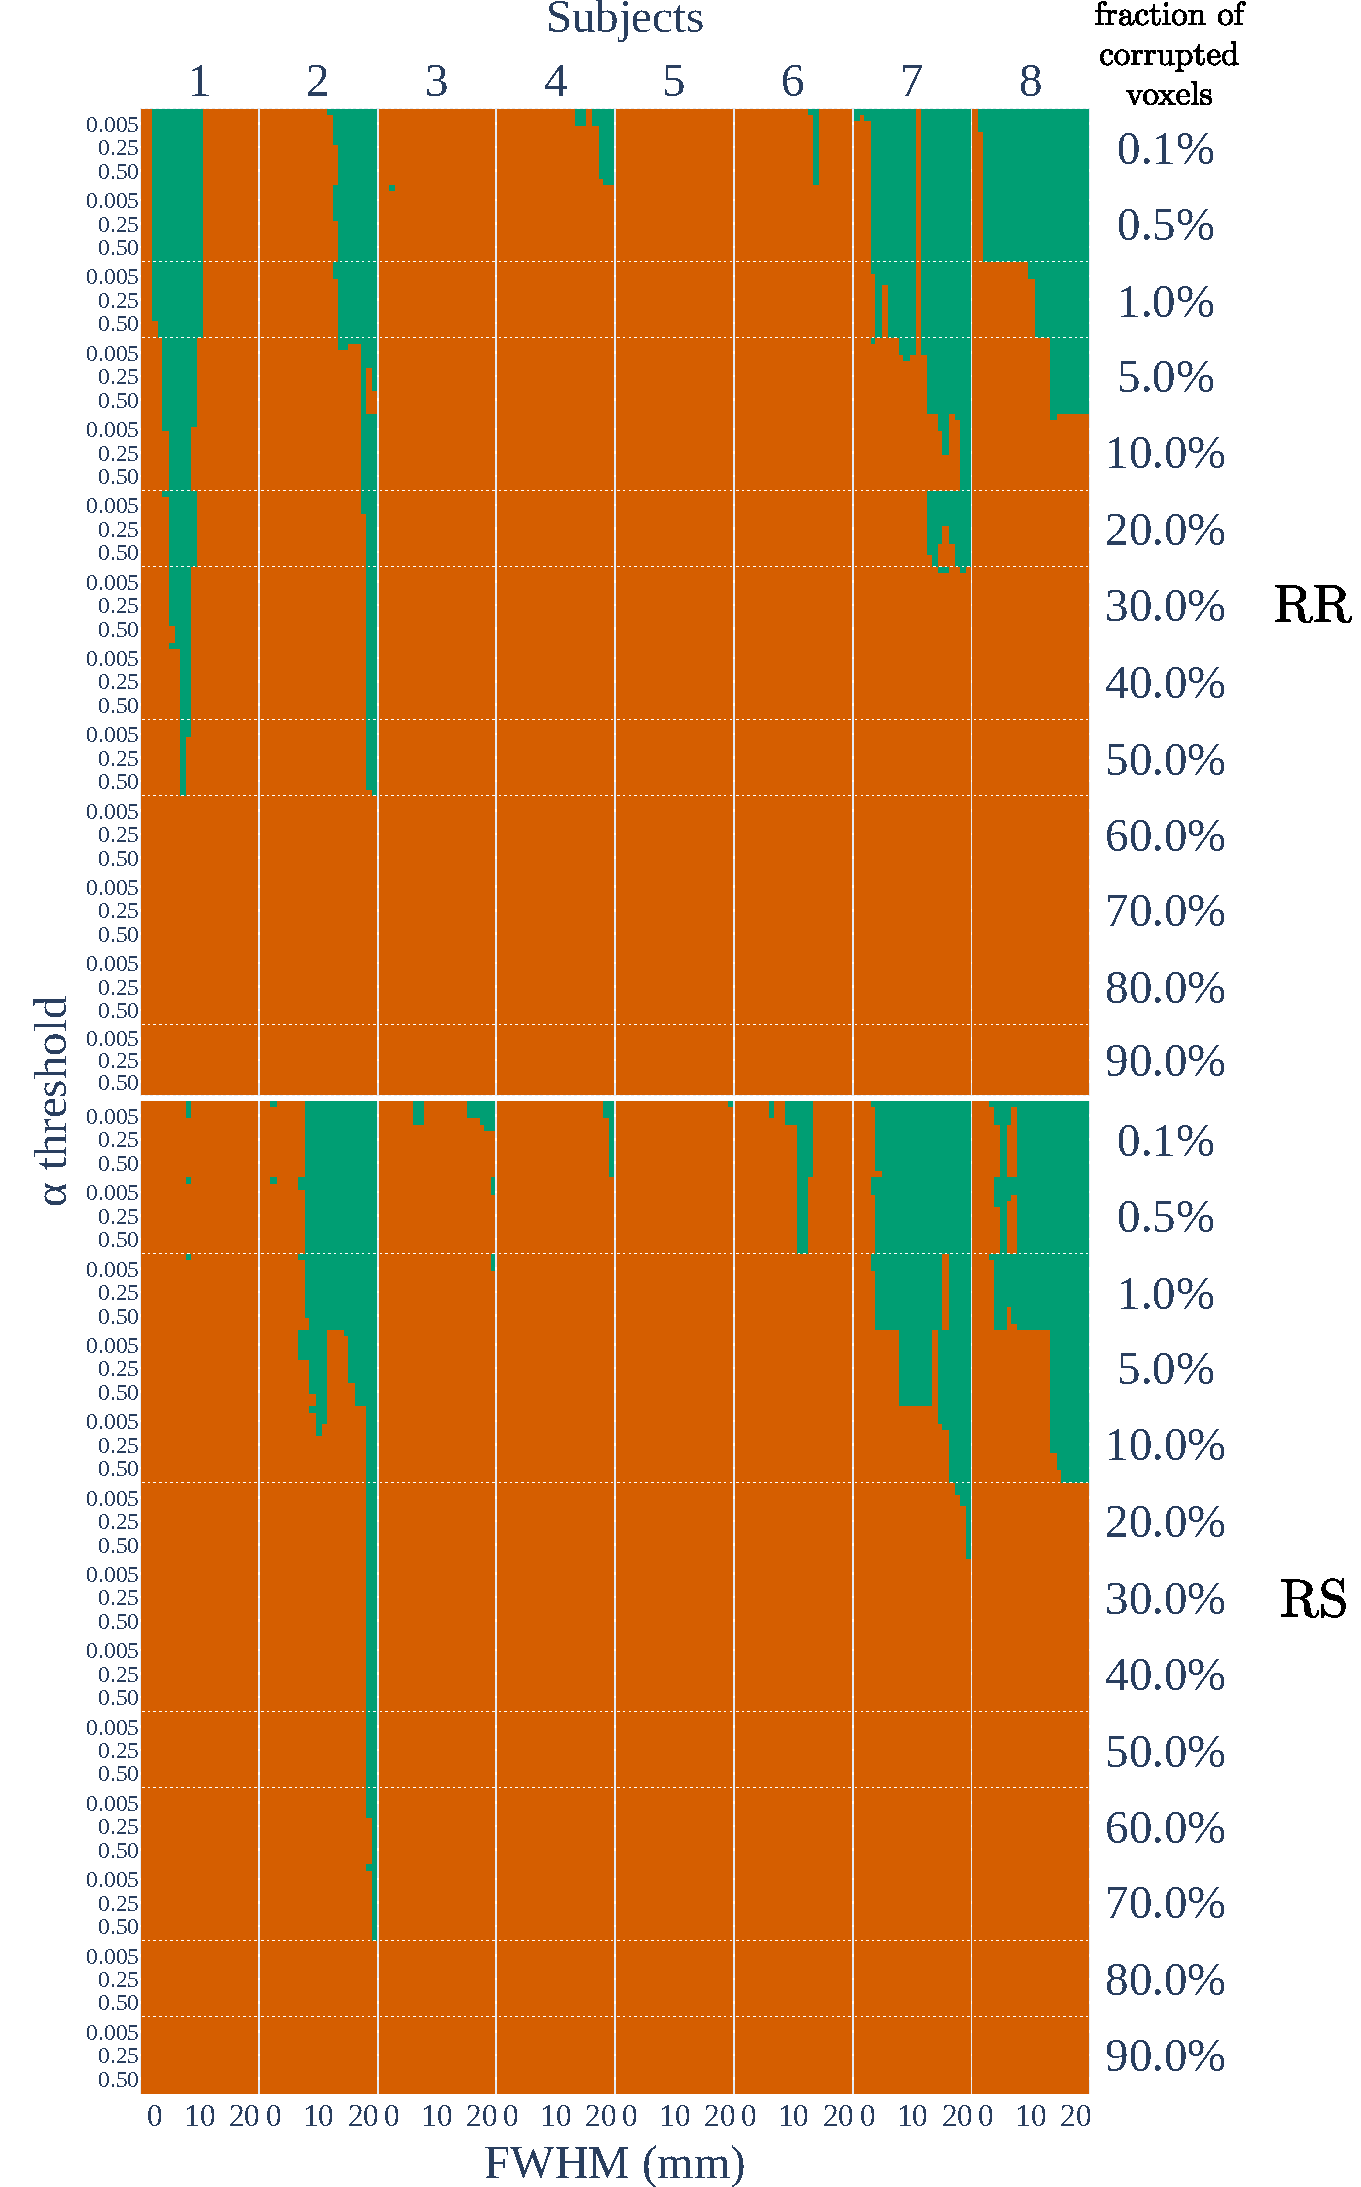
\includegraphics[width=\linewidth]{figures/template/template_fwe_bonferroni.pdf}
    \caption{Corrupted template check for RR (top) and RS (bottom) modes. The stability tests correctly rejected results produced with corrupted templates beyond a subject-dependent threshold of corrupted voxels.}
    \label{fig:template_bonferroni}
\end{figure}

% \subsection{The results stability test accepted CPU architecture variations}

%  The goal was to identify potential sources of variability in \fmriprep results more broadly. First, to test 
% variability across hardware architectures, we executed \fmriprep in IEEE mode in 6 different CPU architectures encountered in different computing clusters of the Digital Alliance of Canada \TG{right?}. The goal of this experiment was to explore whether hardware architecture has a measurable impact on \fmriprep results beyond numerical variability. \TG{Tristan to expand further depending on Yohan's current checks.}


% %  Figure~\ref{fig:arch_bonferroni} shows the results of the stability test for increasing $\alpha$ and FWHM values for RR and RS. We see that the architecture used has no impact on the stability test since results are identical across architecture for a subject and a perturbation mode given. For subject 1, we see that the variability of the stability test results is more important across perturbation modes.
% % In conclusion, the mode of perturbation used in constructing the test holds greater significance than the utilized architecture. This suggests that \fmriprep has low usage of specific hardware instructions, leading to a significant reduction in the variability generated across different architectures.

% \begin{figure}
%     \centering
%     \includegraphics[width=\linewidth]{figures/arch/arch_fwe_bonferroni.pdf}
%     \caption{Stability test application to different CPU architectures for subjects 1 to 8. \TG{Mention RR and RS in the figure.} \TG{Mention which architecture was used to build the test} A: AMD Rome 7532; B: Intel E5-2683 v4 Broadwell; C: Intel Silver 4216 Cascade Lake; D: Intel Platinum 8160F Skylake; E: Intel Gold 5120 Skylake; F: Intel Gold 6238 Cascade Lake.}
%     \label{fig:arch_bonferroni}
% \end{figure}

\subsection{The results stability test detected subtle updates in \fmriprep image processing methods}

The previous sanity checks demonstrated a satisfying level of sensitivity and specificity of our stability test for simple scenarios. Subsequently, we applied it to our main motivating use case: the detection of results differences in \fmriprep LTS versions. We tested the results produced by different versions of \fmriprep, having built the results stability test for version 20.2.1. The goal of this experiment was to evaluate the ability of the stability test to detect significant software updates in \fmriprep. The stability test accepted results produced by versions 20.2.0 to 20.2.4 for all subjects (Figure~\ref{fig:version_bonferroni}). However, the test rejected results produced by versions 20.2.5 and onwards, suggesting a substantial change in the analysis methods from version 20.2.5. Investigations with the \fmriprep developers revealed that the interpolation scheme involved in the resampling of the segmented brain maps from MGZ format into NiFTI was changed in version {20.2.5} from trilinear interpolation to nearest neighbor (see PR \href{https://github.com/nipreps/smriprep/pull/268}{\url{github.com/nipreps/smriprep/pull/268}}). The ability of our results stability test to detect such subtle changes in the analysis supports its relevance in the release process of long-term support data analysis software.

\begin{figure}
    \centering
    \includegraphics[width=\linewidth]{figures/fmriprep-versions/versions_fwe_bonferroni.pdf}
    \caption{Stability test application to different \fmriprep versions.}
    \label{fig:version_bonferroni}
\end{figure}


\section{Discussion}

% summary of results

We proposed the first approach to build results stability tests for data analyses using numerical variability. This approach does not require an exact solution, a reference solution, or even an acceptable bound of variation around the computed solution. We applied this approach to \fmriprep, one of the largest processing pipelines in neuroimaging, and we demonstrated its ability to detect subtle algorithmic updates in \fmriprep versions while remaining specific enough to accept numerical variations within a reference version of the application. Overall, our results stability test is a practical tool that can be readily integrated into the \fmriprep development environment. \TG{here it would be nice to give pointers on how to use it}

% \subsection*{Statistical test}
Designing the results stability test involved multiple choices that we discuss hereafter.
First, we employed a parametric statistical test (Equation~\ref{eq:pval}) that is less compute-intensive than non-parametric methods that typically demand larger sample sizes --- in our case, more than $100$ repetitions per subject --- to achieve acceptable confidence levels ($\geq 0.95$).
Indeed, the computing and storage costs required to apply stochastic arithmetic to neuroimaging tools such as \fmriprep are high, although they are incurred only during the construction of the test
and not during its evaluation, which therefore does not impact test users. Moreover, our stability test operates at the level of individual voxels and is accepted or rejected globally for a given image. Refining the test by regions of interest in the image could provide additional insights about the application behavior.

% \subsection*{Perturbation modes}
% Can be applied to any scientific software using libm functions
% Generates variability comparable to Random Seed
% True for neuroimaging but not necessarily for other application domains.
% For those domains (where libm is not sufficient to explain variability) we need to instrument other computations regions.
The random rounding method adopted to sample the null distribution of results produced by the reference application can be applied regardless of the type of input and output data involved. In our \fmriprep use case, random rounding resulted in variability comparable to the one obtained from varying the random seed, which increased the confidence in our results. However, random rounding and random seed are different types of perturbations and there is no guarantee that they would produce comparable variability patterns in general. We applied random rounding to functions of the GNU libmath library, since previous experiments had shown that neuroimaging analyses commonly rely on these functions. Other types of applications may require that random rounding be applied to other libraries. For instance, the work in~\cite{pepe2022numerical} reports on the use of random rounding for deep neural networks, which required instrumenting the entire Tensorflow application and its dependencies.

%\subsection*{Pre-processing (smoothing)}
The size of the spatial smoothing kernel had a notable impact on the performance of the stability test. Smoothing was required for the test to accept results produced by the reference application and therefore reach an acceptable level of specificity. Smoothing gaussianizes voxel intensity distributions and therefore tends to make them respect the main assumption of the test. Smoothing is a very common operation in neuroimage analysis, however, FWHM values usually remain lower than 8mm while our test required 15mm for most subjects. It would be interesting to further investigate why such large smoothing kernel sizes were required, since large smoothing kernel sizes reduce the sensitivity of our test.

%\subsection*{Dataset}
The results stability test behaved quite differently across the 8 test subjects, which motivates the inclusion
of a variety of different datasets in such test cases. To build our test, we selected subjects to reflect diverse acquisition parameters, resolutions, ages, and sexes.

% The diversity is reflected in the numerical stability of the results that vary considerably from subject to subject.
% Despite these differences, our stability test demonstrated robustness across the heterogeneously quality data, exhibiting a wide range of valid configurations $\alpha$ and FWHM among subjects.

% \subsection*{Multiple comparisons}
The Bonferroni correction for multiple comparisons is conservative in our case given that the voxel intensities in a brain image are not independent.
Possible alternatives to this correction are presented in~\cite{NICHOLS2007246}. The use of Bonferroni correction reduces the sensitivity of our test
and increases its specificity.


% , meaning that it tends to be very sensitive and poorly specific.
% Hence, our test should be very permissive by failing to catch images falling outside of the reference distribution (true positive).
% However, this is not what we observed in practice as the LOO check demonstrated. We see two main reasons for that.
% First, Bonferroni correction assumes that the multiple tests are independent, which is not the case for the voxels that are spatially correlated.
% Second, neuroimaging pre-processing pipelines involve optimization steps for spatial normalization and bias field correction.
% These procedures are known to be highly sensitive to numerical perturbations~\cite{clarenz2006computational}, resulting in normalized images with
% different geometric solutions where white/grey matter borders are specifically unstable (Figure~\ref{fig:uncertainty-maps-0mm-disc}).
% Voxels at these borders have intensities transitioning from grey to white matter, making the voxel-wise analysis difficult. This requires a good sampling of the solution space which is difficult due to its high dimensionality. One way to mitigate this phenomenon is to take into account local information in the neighborhood of a voxel, by computing the covariance matrix for instance. This would however lead to change our statistical assumptions by working with multivariate Gaussian distributions.


%\subsection*{Future work}
In future work, we plan to extend our methodology to other data types and investigate its applicability under different statistical hypotheses.
Results stability tests could be applied to diverse scientific domains beyond neuroimaging, further enhancing the reliability and reproducibility of computational results. In the short term, we plan to extend our test to functional neuroimaging data, which involves 4D images.


\section*{Acknowledgments}

Computations were made on the Narval supercomputer from \'Ecole de Technologie
Sup\'erieure (ETS, Montr\'eal), managed by Calcul Québec and the Digital Research Alliance of Canada. The
operation of this supercomputer is funded by the Canada Foundation for
Innovation (CFI), Ministère de l’Économie, des Sciences et de l’Innovation du
Québec (MESI) and le Fonds de recherche du Québec – Nature et technologies
(FRQ-NT).

\bibliographystyle{IEEEtran}
\bibliography{main}

\appendix

\section*{Numerical variability results for different smoothing kernel sizes}
\label{appendix:numerical_uncertainty}

% \begin{landscape}
%     \begin{figure}
%         \vspace*{-2cm}
%         \centering
%         \uncertaintyMap{0}{1}{ds000256}{sub-CTS201}[true] \\
%         \uncertaintyMap{0}{2}{ds000256}{sub-CTS210} \\
%         \uncertaintyMap{0}{3}{ds001600}{sub-1} \\
%         \uncertaintyMap{0}{4}{ds001748}{sub-adult15} \\
%         \uncertaintyMap{0}{5}{ds001748}{sub-adult16} \\
%         \uncertaintyMap{0}{6}{ds001771}{sub-36} \\
%         \uncertaintyMap{0}{7}{ds002338}{sub-xp201} \\
%         \uncertaintyMap{0}{8}{ds002338}{sub-xp207} \\
%         \includegraphics*[width=.7\linewidth]{figures/colorbar_sigbit.pdf}
%         \caption{Uncertainty measured for subjects 1 to 8 (from top to bottom) across n=30 perturbed samples, with FWHM=0mm. }
%         \label{fig:uncertainty-maps-0mm}
%     \end{figure}
% \end{landscape}

% \begin{landscape}
%     \begin{figure}
%         \vspace*{-2cm}
%         \centering
%         \uncertaintyMap{5}{1}{ds000256}{sub-CTS201}[true] \\
%         \uncertaintyMap{5}{2}{ds000256}{sub-CTS210} \\
%         \uncertaintyMap{5}{3}{ds001600}{sub-1} \\
%         \uncertaintyMap{5}{4}{ds001748}{sub-adult15} \\
%         \uncertaintyMap{5}{5}{ds001748}{sub-adult16} \\
%         \uncertaintyMap{5}{6}{ds001771}{sub-36} \\
%         \uncertaintyMap{5}{7}{ds002338}{sub-xp201} \\
%         \uncertaintyMap{5}{8}{ds002338}{sub-xp207} \\
%         \includegraphics*[width=.7\linewidth]{figures/colorbar_sigbit.pdf}
%         \caption{Uncertainty measured for subjects 1 to 8 (from top to bottom) across n=30 perturbed samples, with FWHM=5mm. }
%         \label{fig:uncertainty-maps-5mm}
%     \end{figure}
% \end{landscape}

% \begin{landscape}
%     \begin{figure}
%         \vspace*{-2cm}
%         \centering
%         \uncertaintyMap{10}{1}{ds000256}{sub-CTS201}[true] \\
%         \uncertaintyMap{10}{2}{ds000256}{sub-CTS210} \\
%         \uncertaintyMap{10}{3}{ds001600}{sub-1} \\
%         \uncertaintyMap{10}{4}{ds001748}{sub-adult15} \\
%         \uncertaintyMap{10}{5}{ds001748}{sub-adult16} \\
%         \uncertaintyMap{10}{6}{ds001771}{sub-36} \\
%         \uncertaintyMap{10}{7}{ds002338}{sub-xp201} \\
%         \uncertaintyMap{10}{8}{ds002338}{sub-xp207} \\
%         \includegraphics*[width=.7\linewidth]{figures/colorbar_sigbit.pdf}
%         \caption{Uncertainty measured for subjects 1 to 8 (from top to bottom) across n=30 perturbed samples, with FWHM=10mm. }
%         \label{fig:uncertainty-maps-10mm}
%     \end{figure}
% \end{landscape}

% \begin{landscape}
%     \begin{figure}
%         \vspace*{-2cm}
%         \centering
%         \uncertaintyMap{20}{1}{ds000256}{sub-CTS201}[true] \\
%         \uncertaintyMap{20}{2}{ds000256}{sub-CTS210} \\
%         \uncertaintyMap{20}{3}{ds001600}{sub-1} \\
%         \uncertaintyMap{20}{4}{ds001748}{sub-adult15} \\
%         \uncertaintyMap{20}{5}{ds001748}{sub-adult16} \\
%         \uncertaintyMap{20}{6}{ds001771}{sub-36} \\
%         \uncertaintyMap{20}{7}{ds002338}{sub-xp201} \\
%         \uncertaintyMap{20}{8}{ds002338}{sub-xp207} \\
%         \includegraphics*[width=.7\linewidth]{figures/colorbar_sigbit.pdf}
%         \caption{Uncertainty measured for subjects 1 to 8 (from top to bottom) across n=30 perturbed samples, with FWHM=20mm. }
%         \label{fig:uncertainty-maps-20mm}
%     \end{figure}
% \end{landscape}


\begin{landscape}
    \begin{figure}
        \vspace*{-2cm}
        \centering
        \uncertaintyMapDiscrete{0}{1}{ds000256}{sub-CTS201}[true] \\
        \uncertaintyMapDiscrete{0}{2}{ds000256}{sub-CTS210} \\
        \uncertaintyMapDiscrete{0}{3}{ds001600}{sub-1} \\
        \uncertaintyMapDiscrete{0}{4}{ds001748}{sub-adult15} \\
        \uncertaintyMapDiscrete{0}{5}{ds001748}{sub-adult16} \\
        \uncertaintyMapDiscrete{0}{6}{ds001771}{sub-36} \\
        \uncertaintyMapDiscrete{0}{7}{ds002338}{sub-xp201} \\
        \uncertaintyMapDiscrete{0}{8}{ds002338}{sub-xp207} \\
        \includegraphics*[width=.7\linewidth]{figures/colorbar_sigbit_discrete.pdf}
        \caption{Numerical variability measured for subjects 1 to 8 (from top to bottom) across n=30 perturbed samples, with FWHM=0mm. }
        \label{fig:uncertainty-maps-0mm-disc}
    \end{figure}
\end{landscape}

\begin{landscape}
    \begin{figure}
        \vspace*{-2cm}
        \centering
        \uncertaintyMapDiscrete{5}{1}{ds000256}{sub-CTS201}[true] \\
        \uncertaintyMapDiscrete{5}{2}{ds000256}{sub-CTS210} \\
        \uncertaintyMapDiscrete{5}{3}{ds001600}{sub-1} \\
        \uncertaintyMapDiscrete{5}{4}{ds001748}{sub-adult15} \\
        \uncertaintyMapDiscrete{5}{5}{ds001748}{sub-adult16} \\
        \uncertaintyMapDiscrete{5}{6}{ds001771}{sub-36} \\
        \uncertaintyMapDiscrete{5}{7}{ds002338}{sub-xp201} \\
        \uncertaintyMapDiscrete{5}{8}{ds002338}{sub-xp207} \\
        \includegraphics*[width=.7\linewidth]{figures/colorbar_sigbit_discrete.pdf}
        \caption{Numerical variability measured for subjects 1 to 8 (from top to bottom) across n=30 perturbed samples, with FWHM=5mm. }
        \label{fig:uncertainty-maps-5mm-disc}
    \end{figure}
\end{landscape}

\begin{landscape}
    \begin{figure}
        \vspace*{-2cm}
        \centering
        \uncertaintyMapDiscrete{10}{1}{ds000256}{sub-CTS201}[true] \\
        \uncertaintyMapDiscrete{10}{2}{ds000256}{sub-CTS210} \\
        \uncertaintyMapDiscrete{10}{3}{ds001600}{sub-1} \\
        \uncertaintyMapDiscrete{10}{4}{ds001748}{sub-adult15} \\
        \uncertaintyMapDiscrete{10}{5}{ds001748}{sub-adult16} \\
        \uncertaintyMapDiscrete{10}{6}{ds001771}{sub-36} \\
        \uncertaintyMapDiscrete{10}{7}{ds002338}{sub-xp201} \\
        \uncertaintyMapDiscrete{10}{8}{ds002338}{sub-xp207} \\
        \includegraphics*[width=.7\linewidth]{figures/colorbar_sigbit_discrete.pdf}
        \caption{Numerical variability measured for subjects 1 to 8 (from top to bottom) across n=30 perturbed samples, with FWHM=10mm. }
        \label{fig:uncertainty-maps-10mm-disc}
    \end{figure}
\end{landscape}

\begin{landscape}
    \begin{figure}
        \vspace*{-2cm}
        \centering
        \uncertaintyMapDiscrete{20}{1}{ds000256}{sub-CTS201}[true] \\
        \uncertaintyMapDiscrete{20}{2}{ds000256}{sub-CTS210} \\
        \uncertaintyMapDiscrete{20}{3}{ds001600}{sub-1} \\
        \uncertaintyMapDiscrete{20}{4}{ds001748}{sub-adult15} \\
        \uncertaintyMapDiscrete{20}{5}{ds001748}{sub-adult16} \\
        \uncertaintyMapDiscrete{20}{6}{ds001771}{sub-36} \\
        \uncertaintyMapDiscrete{20}{7}{ds002338}{sub-xp201} \\
        \uncertaintyMapDiscrete{20}{8}{ds002338}{sub-xp207} \\
        \includegraphics*[width=.7\linewidth]{figures/colorbar_sigbit_discrete.pdf}
        \caption{Numerical variability measured for subjects 1 to 8 (from top to bottom) across n=30 perturbed samples, with FWHM=20mm. }
        \label{fig:uncertainty-maps-20mm-disc}
    \end{figure}
\end{landscape}


% \section{Colors Palette}
% Fail: \texttt{\#D55E00}
% Pass: \texttt{\#009E73}

% \section{Results for uncorrected tests}
% \label{appendix:multiple-comparison-tests}

% In the absence of multiple comparison corrections, we expect
% by construction to incorrectly reject each $H_{0,i}$ with probability $\alpha$ a.k.a
% the per-comparison error rate (PCER). To account for the PCER, we measure the
% fraction of positive z-tests $V_P$ among the $v$ voxels in the image and the
% tested \fmriprep result is considered part of the reference distribution iif:
% \begin{equation}
%     V_{P} \leq \alpha.
%     \label{eqn:pce}
% \end{equation}

% For each of the $n$ repetitions,
% we measured $V_P$, the fraction of
% positive z-tests among the $v$ voxels as well as $\mathds{1}_n$, the number of repetitions
% that passed the test with Bonferroni correction.

% For the uncorrected tests (Equation~\ref{eqn:pce}), we expect $\overline{V_P}$ to have
% the following upper bound:
% \[
%     \overline{V_P} \leq
%     \alpha  + t_{29,0.05} \frac{\tilde{\sigma}_{V_P}}{\sqrt{30}}
% \]
% with
% $t_{k,\gamma}$ the $(1-\gamma)$quantile of the Student distribution with $k$ degrees of freedom,
% and $\overline{V_P}$ and $\tilde{\sigma}_{V_P}$ the mean and standard-deviation estimated from
% $n$ $V_P$ measures.
% This confidence interval is obtained from a two-tailed one-sample
% t-test with $n-1$ degrees of freedom at a level of significance $\alpha_0=0.05$:
% \[
%     \mathbb{P}
%     \left(
%     -t_{n-1,\alpha_0/2}
%     <
%     \dfrac{\overline{V_p} - \alpha}{\tilde{\sigma}_{V_P} / \sqrt{n}}
%     <
%     t_{n-1,\alpha_0/2}
%     \right)
%     = 1 - \alpha_0
% \]

% fraction of positive
% z-tests $V_P$ among the $v$ voxels should be close to the nomimal value $\alpha$
% on average. To assess the validity of our LOO test, we test that the average
% of the $n$ $V_P$ fractions measured belongs to a confidence interval
% around the nomimal value $\alpha$. To do so, we use  resulting in the
% following confidence interval for $V_P$:

% obtained from:

% \begin{figure}
%     \centering
%     \includegraphics[width=\linewidth]{figures/inter-subject/inter_pce.pdf}
%     \caption{Inter-subject check for the uncorrected test for RR (top) and RS (bottom) modes. We expect that the tests would pass along the diagonals and be rejected otherwise.
%         Out of a total of 17,472 individual assessments, we reported 791 failures in the RR mode, representing a failure rate of 0.05\%, and 685 failures in the RS mode, corresponding to a failure rate of 0.04\%. These data corroborate our test's capacity to discern inter-subject variability.
%     }
%     \label{fig:ieee-check-pce}
% \end{figure}


% \begin{figure}
%     \centering
%     \includegraphics[width=\linewidth]{figures/fmriprep-versions/versions_pce.pdf}
%     \caption{Uncorrected test applications on different \fmriprep versions.}
%     \label{fig:versions_pce}
% \end{figure}

% \begin{figure}
%     \centering
%     \includegraphics[width=\linewidth]{figures/arch/arch_pce.pdf}
%     \caption{Uncorrected test applications on CPU architectures.}
%     \label{fig:arch_pce}
% \end{figure}


% \section{Uncertainty maps for others FWHM}

% \begin{figure}
%     \centering
%     \includegraphics[width=\linewidth]{figures/loo_pce.pdf}
%     \caption{PCE}
%     \label{fig:loo_pce}
% \end{figure}

% \begin{figure}
%     \centering
%     \includegraphics[width=\linewidth]{figures/template/template_pce.pdf}
%     \caption{Corrupted template check for RR and RS modes (pce)}
% \end{figure}


\end{document}

